\chapter{Evaluation}

With the eventual growth of the Lightning Network a fee market for channel liquidity will emerge. How routing nodes 

\section{Lightning network as a graph}




\section{Fee as a competitive equilibrium}

The

The conventional long run demand and supply curve apply to the fee market.

If a demand is running DD' and Supply SS' and

Suppose the average fee price is set at $F_{1}$ with demand $F_{1}D_{1}$ and supply $F_{1}S_{1}$.

\begin{figure}[!htb]
	\hspace*{-0.7cm} 
	\centering
	\includegraphics[width=11cm]{images/equilibrium_sized.png}
	\caption{ 
		}
		\label{fig:equilibrium}
		\hspace*{2mm} 	
\end{figure}



The cost of procuring a shortest path between s and d might be unequal for two different routing nodes dependent on already existing paths and set policies.

\section{Pricing function}

Betweenness centrality

\[ g(v) = \sum_{s \neq v \neq d}\frac{\sigma_{sd}(v)}{\sigma_{sd}} \]

Steps to find the maximizing the fee profit for outgoing channel $C$ assuming pairs have a uniform probability of conducting a payment.

\begin{enumerate}
	\item Calculate the shortest path from all-to-all vertices without going through $C$ with either Floyd-Warshall or Johnson. 
	\item Calculate shortest path from $C$ source to all explicitly going through $C$ with Dijkstra.
	\item Compare difference between all-to-all cost with all-to-$V$-to-all, producing a cumulative summation over the difference.
	\item Maximizing fee * cumulative difference.
\end{enumerate} 

\section{Topology}

Network topology

\[ P(k) \propto k^{-\gamma} \]

\[ p_i = \dfrac{k_i}{\sum_{j}^{}k_j}  \]


Lightning network consists of nodes playing game

Non routing nodes, cheap as possible and possible as private as possible(?) 

Barabási–Albert model

Does it become scale free

does any channel opening algorithm perform better than another and essentially force the network into a scale free hub-spoke network instead of a mesh network?
 
oaeu
oaeu
aoue
aoeu
aou
aoeu
oa
uao
ue
aoeu
oaue
oaeu
aoeu
aoe
uaoeu aoeu oaeu aoe uaoeu oaeuthnoeuatnh 
aoeu oaeu oeau thnoeutnhoeuaththe thoaeutheoua 
aoeu h
coeauueuoae uoeua croeaghc oeauh eoucreou chregoucr 
coraeugcrg ecuogcroeug e auoe craoecucgcr aoecug ceoeau 


\newpage
\onecolumn

\begin{figure}[!htb]
	\hspace*{-0.7cm} 
	\centering
	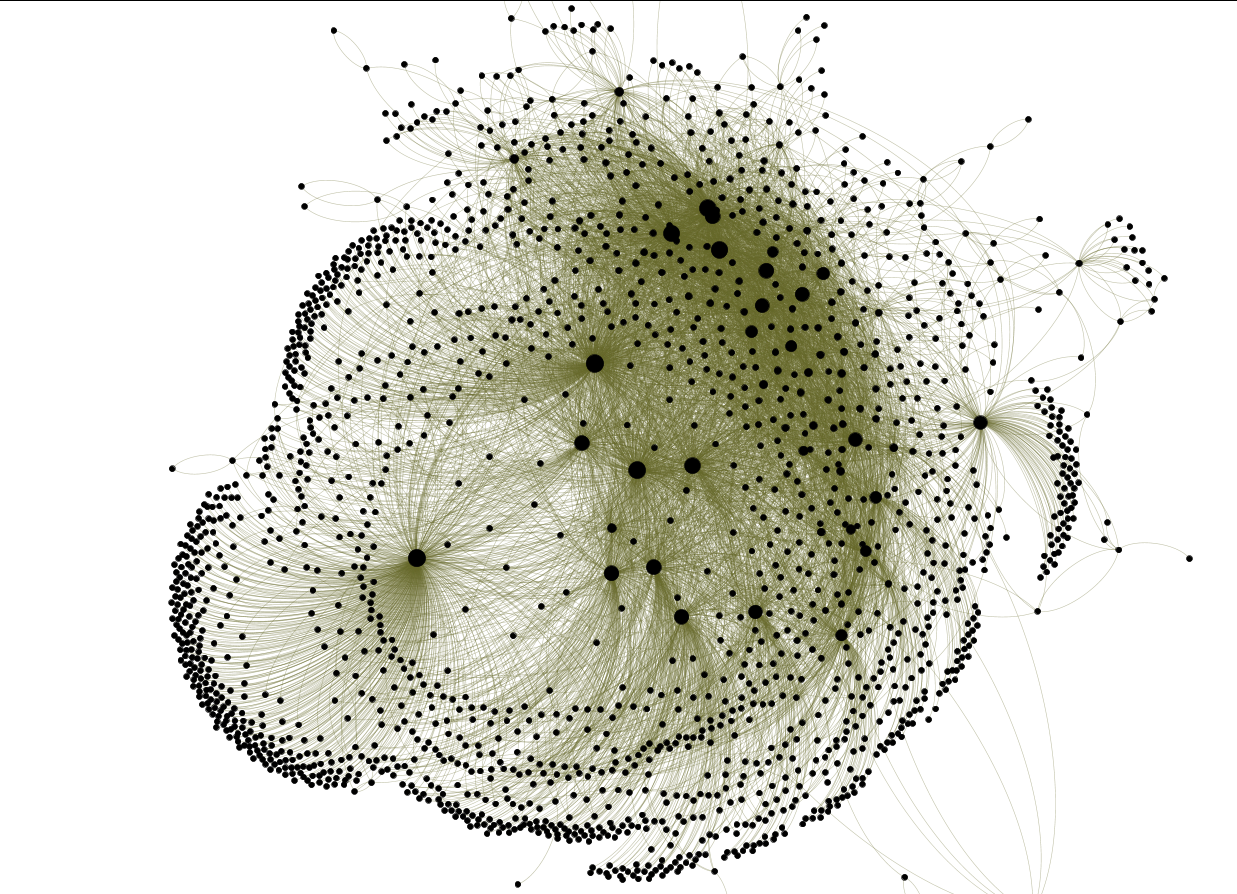
\includegraphics[width=12cm]{graphs/testnet_force.png}
	\vspace*{-0.4cm} 
	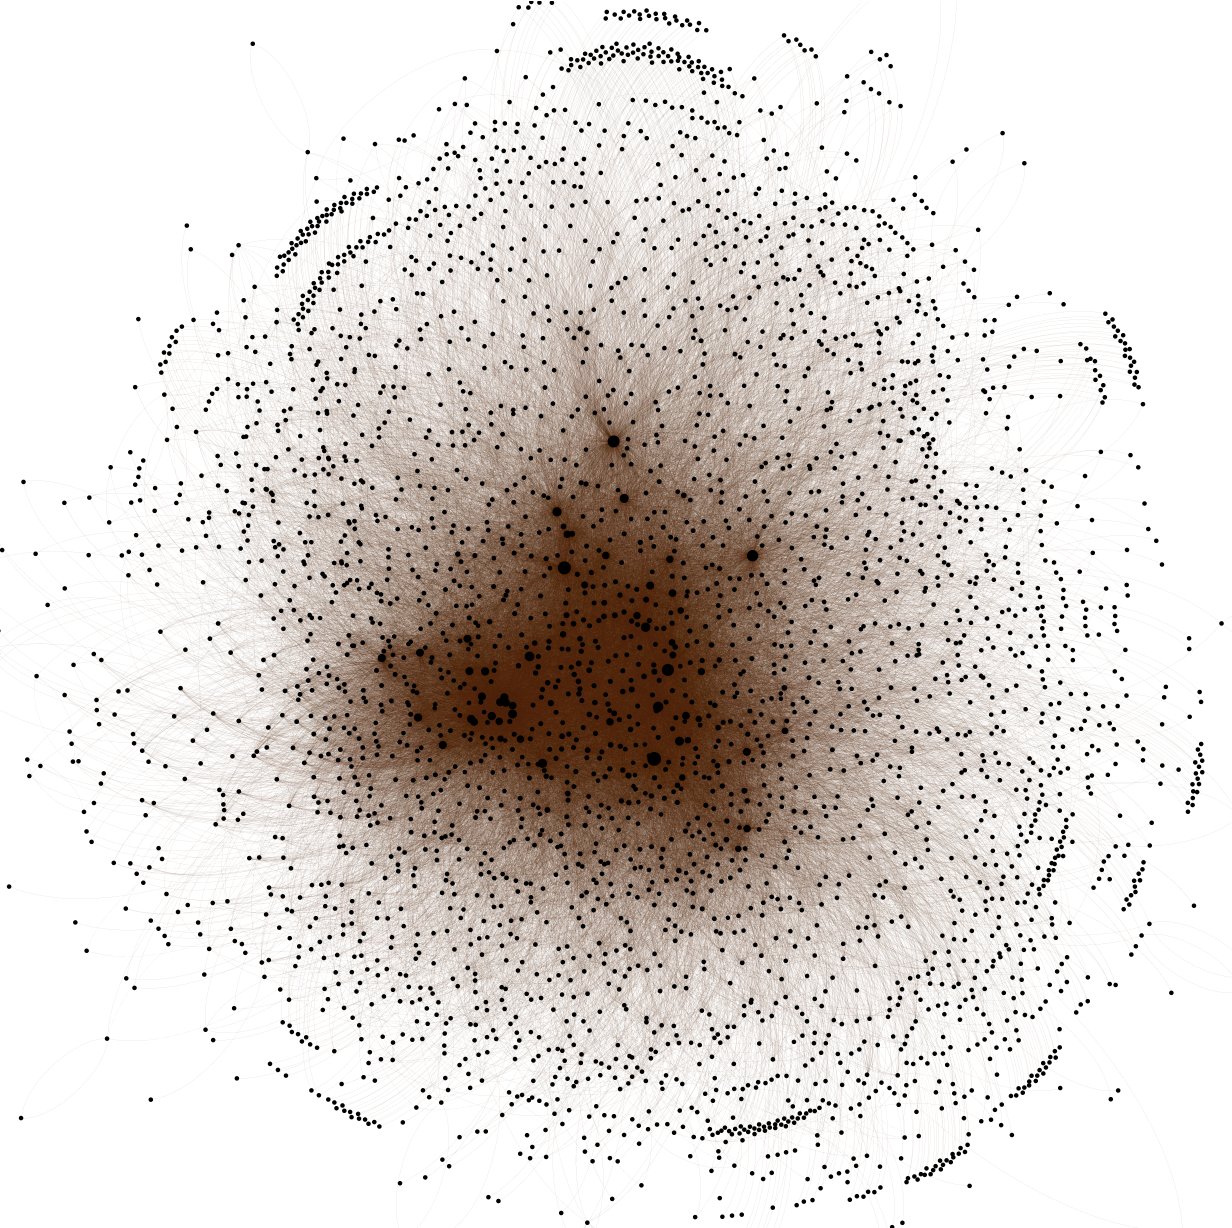
\includegraphics[width=13.6cm]{graphs/mainnet_force3.png}
	\caption{\textit{
		Shows testnet above and mainnet below as of 2019-02-25. Node size corresponds to degree, larger degrees to larger size. Positioning is a mix between Force Atlas and Fruchterman Raingold. Network data retrieved by running a c-lightning node and visualized with Gephi\cite{repository:gephi}.}}
	\label{fig:equilibrium}
	\hspace*{2mm} 	
\end{figure}
\newpage
\twocolumn


% THE ADJUSTABLE SCALE FREE  http://www.uvm.edu/pdodds/files/papers/others/2002/holme2002a.pdf



% https://webusers.imj-prg.fr/~ricardo.perez-marco/publications/articles/antrouting3.pdf

% https://bitfury.com/content/downloads/whitepaper_flare_an_approach_to_routing_in_lightning_network_7_7_2016.pdf

% https://en.wikipedia.org/wiki/Betweenness_centrality